% !TEX root = ./notes.tex
\chapter{Polytropes and the Lane-Emden Equation}

In chapter~\ref{ch.introduction}, we derived an overview of the sun's interior properties. To construct detailed models is clearly an involved task because there are many linked physical variables. For example, the equation of hydrostatic balance, eq.~(\ref{e.hydrostatic}), contains both $\rho$ and $P$; in order to connect these two variables we have to know the temperature, so in general we need in include an equation for heat transport.  Before diving into all that, however, we'll take a little digression to solve some simplified stellar models known as \textbf{polytropes}; these are useful not only for historical reasons, but they also allow for quick analytical calculations.

\section{Historical Background}\label{s.LE-background}

To understand where the term polytropic comes from, let's first consider an ideal gas in hydrostatic equilibrium, and furthermore suppose that the temperature and density lie along an adiabat.  In that case we have the following relations:
\begin{equation}\label{e.ideal-adiabatic-relations} 
T\rho^{1-\gamma} = \mathrm{const};\quad P\rho^{-\gamma} = \mathrm{const};\quad TP^{(1-\gamma)/\gamma} = \mathrm{const},
\end{equation}
which you will recall from elementary thermodynamics. Here $\gamma = C_{P}/C_{\rho}$ is the ratio of specific heats. The equation of state is
\begin{equation}\label{e.ideal-eos}
P = \left(\frac{\NA\kB}{\mu}\right)\rho T,
\end{equation}
where $\mu$ is the mean molecular weight and the quantity in parenthesis is $C_{P}-C_{\rho} = \NA\kB/\mu$.
We might imagine, for example, a rising plume of hot air in Earth's atmosphere.  There is one snag with this analysis for the troposphere, however: the condensation of water vapor means that one cannot hold $\dif s = 0$ in a rising plume of hot air.  Attempting to model this moist convection in the Earth's troposphere motivated work in the early 1900's by Kelvin, Lane, Emden, and others to consider a more general problem, in which $T\dif s = C\dif T$, where $C$ is a constant.  A configuration for which this is true is called \textbf{polytropic}. An adiabat is a special case of a polytrope with $C = 0$. Writing the first law of thermodynamics as $T\dif s = C_{\rho}\dif T -(P/\rho^{2})\dif \rho$, substituting for $T\dif s$, and using equation~(\ref{e.ideal-eos}), we obtain
\[
\left(C_{\rho}-C\right)\frac{\dif T}{T} = \left( C_{P} - C_{\rho}\right)\frac{\dif\rho}{\rho}.
\]
This equation has a solution $T  \propto  \rho^{(C_{P}-C_{\rho})/(C_{\rho}-C)}$. Comparing this solution with equation~(\ref{e.ideal-adiabatic-relations}), we can define a \emph{polytropic exponent}, $\gamma' = (C_{P}-C)/(C_{\rho}-C)$. Then equation~(\ref{e.ideal-adiabatic-relations}) holds with $\gamma$ replaced by $\gamma'$.  The advantage of this approximation is that it relates density to pressure so that one can solve the equation of hydrostatic equilibrium without simultaneously having to solve for $T(r)$.

\section{The Lane-Emden Equation and Solution}\label{s.LE-solution}

To use the polytropic equation of state, write the pressure $P$ as
\begin{equation}\label{e.polytope}
P(r) = K\rho^{1+1/n}(r)
\end{equation}
where $n$ and $K$ are constants. Further define the dimensionless variable $\theta$ via
\begin{equation}\label{e.theta-def}
\rho(r) = \rho_{c}\theta^{n}(r),
\end{equation}
where the subscript $c$ denotes the central value at $r=0$. Note that since
\[ P(r) \propto \rho \times \rho^{1/n} \propto \rho \theta, \]
the quantity $\theta$ plays the role of a dimensionless temperature for an ideal non-degenerate gas.

Substitute equations~(\ref{e.polytope}) and (\ref{e.theta-def}) into Poisson's equation,
\begin{equation}
\nabla^{2}\Phi = 4\pi G\rho,
\end{equation}
and the equation for hydrostatic equilibrium, 
\begin{equation}
\grad P = -\rho\grad \Phi,
\end{equation}
to obtain the \emph{Lane-Emden} equation for index $n$,
\begin{equation}\label{e.LE}
\xi^{-2} \frac{d}{d\xi}\left(\xi^{2}\frac{d\theta}{d\xi}\right) = -\theta^{n}.
\end{equation}
Here $\xi = r/r_{n}$ is the dimensionless coordinate, and
\begin{equation}\label{e.LE-length-scale}
r_{n} = \left[\frac{(n+1)P_{c}}{4\pi G\rho_{c}^{2}}\right]^{1/2}
\end{equation}
is the radial length scale.

For a stellar model described by a single polytropic relation, the appropriate boundary conditions are
\begin{eqnarray}
\label{e.thetabc}\left.\theta(\xi)\right|_{\xi = 0} &=& 1,\\
\label{e.thetapbc}\left.\theta'(\xi)\right|_{\xi=0} &=& 0.
\end{eqnarray}
From the form of equation~(\ref{e.LE}), it follows that $\theta(-\xi) = \theta(\xi)$, that is, the solution is \emph{even} in $\xi$. A power-series solution of $\theta$ out to order $\xi^{6}$ is
\begin{equation}\label{e.series}
\theta(\xi) = 1 - \frac{1}{6}\xi^{2} + \frac{n}{120}\xi^{4} - \frac{n(8n-5)}{15120}\xi^{6} + \mathcal{O}(\xi^{8})
\end{equation}
There are analytical solutions for $n = 0$, 1, and 5:
\begin{eqnarray}
\theta_{0}(\xi) &=& 1-\frac{\xi^{2}}{6}\label{e.solution-0}\\
\theta_{1}(\xi) &=& \frac{\sin\xi}{\xi}\label{e.solution-1}\\
\theta_{5}(\xi) &=& \left(\frac{3}{3 + \xi^{2}}\right)^{1/2}.\label{e.solution-5}
\end{eqnarray}
Finally, the radius of the stellar model is determined by the location of the first zero, $\xi_{1}$.  For example, if $n = 0$ (eq.~[\ref{e.solution-0}]), $\xi_{1} = \sqrt{6}$. Note that if $n=5$ there is no root; the configuration extends to $\xi \to \infty$.  A sample of Lane-Emden solutions is shown in Figure~\ref{f.LE-solutions}.

\begin{figure}[htbp]
\centering{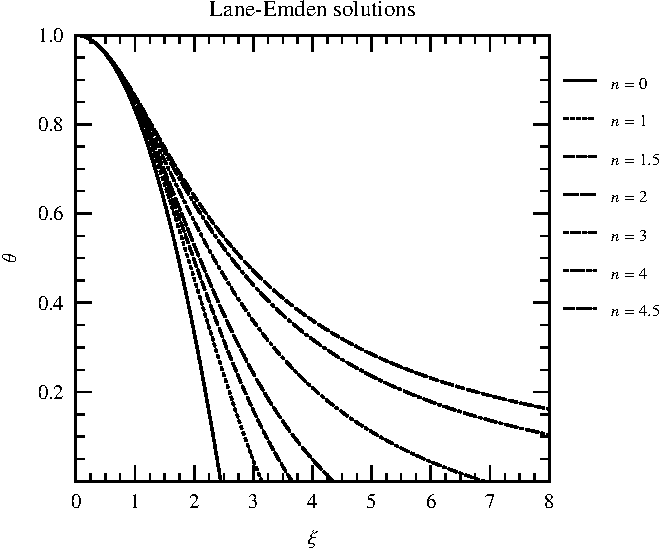
\includegraphics[width=4in]{LE_all.pdf}}
\caption{Solutions of the Lane-Emden equation for selected valued of the index $n$.}
\label{f.LE-solutions}
\end{figure}

\section{Some Useful Relations}

First, let's get the mass of our polytropic sphere.  To do this, we write the integral
\[ M = \int_{0}^{R} 4\pi r^{2} \rho\,\dif r \]
and make the substitutions $r = r_{n}\xi$, $R = r_{n}\xi_{1}$, and $\rho = \rho_{c}\theta^{n}(\xi)$ to obtain
\[
M = 4\pi r_{n}^{3}\rho_{c}\int_{0}^{\xi_{1}} \xi^{2}\theta^{n}(\xi)\,\dif\xi.
\]
Using equation~(\ref{e.LE}) , the integrand can be written as a perfect differential, so we get
\begin{equation}\label{e.LE-mass}
M = 4\pi r_{n}^{3} \rho_{c}\left(-\xi_{1}^{2} \theta_{1}'\right).
\end{equation}
Here I define the shorthand $\theta_{1}' \equiv \theta(\xi)|_{\xi=\xi_{1}}$.  Substituting $r_{n} = R/\xi_{1}$ and dividing by 3 allows us to get a formula relating the central density to the mean density,
\begin{equation}\label{e.LE-density-ratio}
\rho_{c} = \frac{3M}{4\pi R^{3}}\left(-\frac{\xi_{1}}{3\theta_{1}'}\right).
\end{equation}
For the solutions shown in Figure~\ref{f.LE-solutions}, we have the following values of $\rho_{c}/\bar{\rho}$, as shown in Table~\ref{t.LE-properties}.
As the index $n$ increases, the configuration becomes more and more concentrated toward the center.

\begin{table}[htpb]
\caption{Properties of the Lane-Emden solutions.\label{t.LE-properties}}
\begin{center}
\begin{tabular}{c|rrrrrrr}
\hline
$n$ & 0 & 1.0 & 1.5 & 2.0 & 3.0 & 4.0 & 4.5 \\
\hline\hline
$\xi_{1}$ & 2.449 & 3.142 & 3.654 & 4.353 & 6.897 & 14.972 & 31.836\\
$-\theta_{1}'$ & 0.8165 & 0.3183 & 0.2033 & 0.1272 & 0.04243 & 0.008018 & 0.001715\\
$\rho_{c}/\bar{\rho}$ & 1.00 & 3.29 & 5.99 & 11.41 & 54.18 & 622.4 & 6187.8\\
\hline
\end{tabular}
\end{center}
\end{table}

Starting from equation~(\ref{e.LE-mass}), we can substitute for $r_{n}$ using equation~(\ref{e.LE-length-scale}) and $\rho_{c}$ using equation~(\ref{e.LE-density-ratio}) to get an equation for the central pressure,
\begin{equation}\label{e.LE-PC}
P_{c} = \frac{GM^{2}}{R^{4}} \frac{1}{4\pi(n+1)(-\theta_{1}')^{2}}.
\end{equation}
For an ideal gas, $P_{c} = (\NA\kB/\mu)\rho_{c}T_{c}$ with $\mu$ being the mean molecular weight, we can solve for the central temperature,
\begin{equation}\label{e.LE-TC}
T_{c} = \left(\frac{\mu}{\NA\kB}\right)\left(\frac{GM}{R}\right)\frac{1}{(n+1)\xi_{1}(-\theta_{1}')}.
\end{equation}
Finally, starting from equation~(\ref{e.LE-PC}), substituting for $P_{c}$ using equation~(\ref{e.polytope}), and eliminating $\rho_{c}$ using equation~(\ref{e.LE-density-ratio}), we obtain a relation between mass and radius in terms of $K$ and $n$,
\begin{equation}\label{e.LE-mass-radius}
M^{1-1/n} = \left[\frac{K(n+1)}{G(4\pi)^{1/n}} \xi_{1}^{1+1/n}\left(-\theta_{1}'\right)^{1-1/n} \right] R^{1-3/n}.
\end{equation}
Alternatively, one could use this equation to fit $K$ to a star of known $M$ and $R$.

Finally, we can derive a formula for the gravitational energy of our polytropic sphere.  First, we can integrate the equation for the energy,
\[
E_{\mathrm{grav}} = -G\int_{0}^{M}\frac{m}{r}\,\dif m,
\]
by parts to obtain
\begin{equation}\label{e.polytrope-energy-1}
E_{\mathrm{grav}} = -\frac{GM^{2}}{2R} - \frac{1}{2}\int_{0}^{R}\frac{Gm^{2}}{r^{2}}\,\dif r = -\frac{GM^{2}}{2R} - \frac{1}{2}\int_{0}^{R} \frac{\dif\Phi}{\dif r} m\,\dif r.
\end{equation}
If we define our zero of energy to be such that $\Phi(R) = 0$, then we can integrate by parts again to obtain
\begin{equation}\label{e.polytrope-energy-2}
E_{\mathrm{grav}} = -\frac{GM^{2}}{2R} + \frac{1}{2}\int_{0}^{R} \Phi\,\dif m.
\end{equation}
We can rewrite the equation of hydrostatic equilibrium as
\[ \frac{\dif P}{\dif r} = -\frac{\dif\Phi}{\dif r} \rho \]
and use equation~(\ref{e.polytope}) to eliminate $P$ to obtain
\[ \frac{\dif\Phi}{\dif r} = (1+n) K \rho^{1/n} .\]
Integrating from a point in the star $r$ to $R$, and again using choosing $\Phi(R) = 0$, we obtain
\begin{equation}\label{e.polytrope-energy-3}
\Phi(r) = -(1+n)K\rho(r)^{1/n} = -(1+n)\frac{P(r)}{\rho(r)}.
\end{equation}
Inserting equation~(\ref{e.polytrope-energy-3}) into equation~(\ref{e.polytrope-energy-2}), we have
\begin{equation}\label{e.polytrope-energy-4}
E_{\mathrm{grav}} = -\frac{GM^{2}}{2R} - \frac{1+n}{2}\int_{0}^{M} \frac{P}{\rho}\,\dif m = -\frac{GM}{2R} + \frac{1+n}{6}E_{\mathrm{grav}},
\end{equation}
where we used equation~(\ref{e.virial-1}) to relate the integral of $P/\rho$ to $E_{\mathrm{grav}}$. Solving equation~(\ref{e.polytrope-energy-4}) for $E_{\mathrm{grav}}$ gives us the desired result,
\begin{equation}\label{e.polytrope-energy}
E_{\mathrm{grav}} = -\frac{3}{5-n} \frac{GM^{2}}{R}.
\end{equation}
Note that solutions with $n > 5$ have a positive gravitational energy.

\section{Eddington Standard Model}\label{s.LE-Eddington-Standard-Model}

Polytropes with index $n=3/2$ correspond to fully convective stars ($P \propto \rho^{5/3}$, the relation for an adiabat) or for white dwarfs (non-relativistic, degenerate equation of state). Another interesting case, for historical reasons, is the \emph{Eddington Standard Model}, which is a fair approximation to main-sequence stars with $M \gtrsim M_{\sun}$.  Suppose we write the equation of state as the sum of ideal gas and radiation pressure,
\begin{equation}\label{e.eos-with-rad}
 P  = \frac{\rho\kB T}{\mu \mb} + \frac{1}{3}a T^{4}.
\end{equation}
Now make the \emph{ansatz} that
\begin{equation}\label{e.beta-def}
\frac{P_{\mathrm{rad}}}{P} = \frac{aT^{4}}{3P} = 1-\beta = \mathrm{const.},
\end{equation}
that is, the radiation pressure is a fixed fraction of the total pressure everywhere.
Solving for $T$ in terms of $P$ and $\beta$,
\[ T = \left[\frac{3(1-\beta) P}{a}\right]^{1/4}, \]
and inserting this into equation~(\ref{e.eos-with-rad}) gives us a simple EOS,
\begin{equation}\label{e.beta-eos}
P = \left[\left(\frac{\kB}{\mu\mb}\right)^{4}\frac{3}{a}\right]^{1/3}\left[\frac{1-\beta}{\beta^{4}}\right]^{1/3} \rho^{4/3}.
\end{equation}
This is the equation for a polytrope of index 3.

Why is it at all reasonable to take $\beta$ as being constant? To explore this, go back to the equation for radiative diffusion
\[ F(r) = -\frac{1}{3}\frac{c}{\rho\kappa}\frac{\dif aT^{4}}{\dif r}. \]
Write the flux as $F(r) = L(r)/(4\pi r^{2})$, and since pressure decreases monotonically with radius, write
\[ 
\frac{\dif aT^{4}}{\dif r} = \frac{\dif aT^{4}}{\dif P}\frac{\dif P}{\dif r} = -\rho\frac{Gm(r)}{r^{2}}\frac{\dif aT^{4}}{\dif P}. 
\]
The equation of radiation transport then becomes
\[ L(r) = \frac{4\pi Gm(r) c}{\kappa(r)} \frac{\dif P_{\mathrm{rad}}}{\dif P}. \]
Dividing both sides by $L\cdot M/\kappa_{\mathrm{Th}}$ and rearranging terms,
\begin{equation}\label{e.Prad-P}
 \frac{\dif P_{\mathrm{rad}}}{\dif P} = \left[\frac{L\kappa_{\mathrm{Th}}}{4\pi GMc}\right]\left(\frac{\kappa(r)}{\kappa_{\mathrm{Th}}}\frac{L(r)}{L}\frac{M}{m(r)}\right).
\end{equation}
Here $L$ is the total luminosity of the star and $M$ is the total mass.  The term in $[\,]$ is a constant (the Thomson opacity $\kappa_{\mathrm{Th}}$ doesn't depend on density or temperature) and we define the \emph{Eddington luminosity} as $L_{\mathrm{Edd}}=4\pi GM c/\kappa_{\mathrm{Th}}$.  For the sun, $L_{\mathrm{Edd}} = 1.5\ee{38}\nsp\ergs\usp\second^{-1} = 3.8\ee{4}\nsp L_{\sun}$.  For the term $(\,)$ on the right-hand side, note the $L(r)/m(r)$ is basically the average energy generation rate interior to a radius $r$.  Since nuclear reactions are temperature sensitive, the heating is concentrated toward the stellar center and $L(r)/m(r)$ decreases with radius. For stars like the sun, free-free opacity is dominant, and since the free-free Rosseland opacity goes as $T^{-3.5}$, $\kappa(r)$ increases with radius.  Thus, if the energy generation rate is not too temperature dependent (the reaction $\pt + \pt \to \hydrogen[2]$ goes roughly as $T^{4.5}$ at $T=10^{7}\nsp\K$), then the term in $(\,)$  does not vary strongly with radius, and $\dif P_{\mathrm{rad}}/P$ is indeed roughly constant. 

\section{Exercises}\label{s.LE-exercises}
\begin{enumerate}
\item Derive equations~(\ref{e.LE-mass})--(\ref{e.LE-mass-radius}).

\item Explain what the mass-radius relation, eq.~(\ref{e.LE-mass-radius}), means for the cases $n=1$ and $n=3$.

\item For a fully convective star, how is the polytropic constant $K$ related to the entropy? Derive a formula for $R$ in terms of $M$ and $s$ in this case.  What happens to the star if heat is added to it?

\item Derive an expression for $\beta$ in terms of the mass of the star for the Eddington Standard Model.

\item Consider a polytrope of index $3/2$.
\begin{enumerate}
\item Using the expression for the entropy of an ideal gas (eq.~[\ref{e.sacker-tetrode}]), show that the entropy is indeed constant throughout the star.
\item Use the Lane-Emden solution to compute the specific entropy, per unit mass, in terms of the central temperature $T$ and the stellar mass $M$: $s = s(T_{c},M)$.
\item Now compute the ``gravothermal'' specific heat
\begin{equation}\label{e.cstar}
c_{\star} = T_{c}\frac{\partial s(T_{c},M)}{\partial T_{c}},
\end{equation}
and comment on its physical significance.
\end{enumerate}

\item We will see later that low-mass pre-main-sequence stars (including brown dwarfs) are fully convective and have nearly constant effective temperatures.  Use these facts to model their contraction.  Assume $T_{\mathrm{eff}} = \mathrm{const.}$ and write the equation for energy balance as $L = 4\pi R^{2} \sigma_{\mathrm{SB}} T_{\mathrm{eff}}^{4} = -\dif E/\dif t$, where $E$ refers to the total energy of the pre-main-sequence star. (Why is there a minus sign?)
\begin{enumerate}
\item Starting from this equation, derive an equation for $R(t)$. What is the characteristic timescale for a star to contract? Scale your answer to $T_{\mathrm{eff}} = 3000\nsp\K$ and $M = 0.1\nsp\Msun$, and use an expression for the energy appropriate for a fully convective star (polytrope of index $3/2$).
\item Compare your findings with more elaborate calculations.  You will find a review in \href{http://arxiv.org/abs/astro-ph/0006383}{``Theory of Low-Mass Stars and Substellar Objects,''} G. Chabrier and I. Baraffe, Ann.\ Rev.\ Astron.\ Astrophys.\ \textbf{38:} 337 (2000). 
\item Using appropriate expressions for the central density and temperature, calculate the time required for a star just below the hydrogen burning limit (about $0.07\nsp\Msun$) to contract to a radius such that $\eF(\rho_{c}) = \kB T_{c}$, where $\eF$ is the Fermi energy, and compare with the evolutionary tracks in Chabrier \& Baraffe.
\end{enumerate}
\end{enumerate}
